\section{Auswertung}
\label{sec:Auswertung}
In diesem Abschnitt wird die Filterkurve der Brückenschaltung und die Suszeptibilität von $\text{Dy}_2\text{O}_3$ , $\text{Gd}_2\text{O}_3$ und  $\text{Nd}_2 \text{O}_3$ bestimmt.

\subsection{Theoretische Bestimmung der Suszeptibilität}

Um einen besseren Überblick über die Qualität der aufgenommenen Messwerte zu erhalten, ist es sinnvoll, diese mit den theoretisch berechneten Suszeptibilitäten zu vergleichen.
Dabei wird nach den Hundschen Regeln vorgegangen. \\

Zu beachten ist dabei auch die Orientierungsquantenzahl $m = (-3, \,-2, \,-1, \,0, \,1, \,2, \,3)$, die für Elektronen mit gleichem Spin immer unterschiedlich sein muss.
Für die drei Proben folgt also:

\begin{itemize}
    \item $\text{Nd}_2 \text{O}_3$ besitzt auf der 4f-Schale drei Elektronen, die nach der ersten Hundschen Regel den gleichen Spin $s_\text{i} = \frac{1}{2}$, also kombiniert einen Gesamtspin von $S = \frac{3}{2}$ besitzen.
          Die drei Elektronen müssen sich also in ihrer Orientierungsquantenzahl unterscheiden. 
          Hier folgt ein maximaler Drehimpuls von $L = \sum m_i = 3 + 2 + 1 = 6$, insgesamt also ein Gesamtdrehimpuls von $J = L - S = 6 - \frac{3}{2} = \frac{9}{2}$,
          da die Schale weniger als halb gefüllt ist.
          Damit ergibt sich nach \eqref{eq:lande-faktor} ein Landé-Faktor von $g_\text{J} = \frac{8}{11}$.

    \item Für $\text{Gd}_2\text{O}_3$ wird analog vorgegangen. Mit sieben Elektronen auf der 4f-Schale mit gleichem Spin folgt $S = 3,5$. 
        Da die Anzahl an Elektronen genau gleich der Anzahl unterschiedlicher Orientierungsquantenzahlen ist, ist der Bahndrehimpuls $L = 0$.
        Der Gesamtdrehimpuls ist damit gleich dem Gesamtspin, $J = S = 3,5$ und der Landé-Faktor $g_\text{J} = 2$.

    \item Mit neun Elektronen auf der 4f-Schale besitzt $\text{Dy}_2\text{O}_3$ mehr Elektronen, als es Orientierungsquantenzahlen gibt, zwei der Elektronen haben also einen negativen Spin.
        Damit ergibt sich $S = 2,5$ und ein Bahndrehimpuls von \\ $L = 3 + 2 + 1 + 0 - 1 - 2 - 3 + 3 + 2 = 5$.
        Für den Gesamtdrehimpuls folgt $J = L + S = 7,5$, da die Schale mehr als halb gefüllt ist, für den Landé-Faktor $g_\text{J} = \frac{4}{3}$.
\end{itemize}

Mit der Avogadrokonstanten $N_a$, der Dichte $\rho$ und der molaren Masse $M_\text{mol}$ gilt für die Anzahl der Momente pro Volumen
\begin{equation*}
    N = 2 N_a \dfrac{\rho}{M_\text{mol}} \,,
\end{equation*}
womit sich nach \eqref{eq:susg_J} und den in \autoref{tab:probwertis} aufgetragenen Dichten, molaren Massen sowie der berechneten Anzahl der Momente pro Volumen
die in \autoref{tab:probwertis} dargestellten theoretischen Suszeptibilitäten ergeben.

\begin{table}[H]
    \centering
    \caption{Dichten $\rho$, molare Massen $M_\text{mol}$, berechnete Momente pro Volumen $N$ und die theoretische Suszeptibilität $\chi_{\text{theo}}$.}
    \label{tab:probwertis}
    \begin{tabular}{S S[table-format=1.2] S[table-format=3.2] S[table-format=1.2] S}
      \toprule
      {} & {$\rho \mathbin{/} \unit{\frac{\gram}{{\centi\meter}^3}}$} & {$M_\text{mol} \mathbin{/} \unit{\frac{\gram}{\mol}}$} & {$N \mathbin{/} \unit{\frac{1}{{\centi\meter}^3}} \cdot 10^{28}$}&{$\chi_{\text{theo}}$}  \\
      \midrule
      {$\text{Nd}_2\text{O}_3$}         &           7,24          &         336,48          &           2,59     &{0,00299}       \\
      {$\text{Gd}_2\text{O}_3$}         &           7,40          &         362,50          &           2,46     &{0,01370}       \\
      {$\text{Dy}_2\text{O}_3$}         &           7,80          &         373,00          &           2,52     &{0,02525}       \\
      \bottomrule
    \end{tabular}
\end{table}



\subsection{Untersuchung der Filterkurve}

Für die Filterkurve wurden die folgenden \autoref{tab:tab1} Messadaten aufgenommen, dabei wurde eine 10-fache Verstärkung verwendet.

\begin{table}[H]
    \centering
    \caption{Messwerte zur Filterkurve.}
    \label{tab:tab1}
    \begin{tabular}{S S}
      \toprule
      {$f \mathbin{/} \unit{\kilo\hertz} $} & {$U \mathbin{/} \unit{\milli\volt} $}  \\
      \midrule
            10.01       &   0.5     \\
            12.95       &   0.78    \\
            16.03       &   1.11    \\
            19.03       &   2.73    \\
            20.1        &   4.4     \\
            21.0        &   8.1     \\
            22.7        &   6.9     \\
            21.1        &   8.1     \\
            30.6        &   0.84    \\
            33.0        &   0.6     \\
            36.2        &   0.51    \\
            38.3        &   0.46    \\
            40.0        &   0.4     \\
      \bottomrule
    \end{tabular}
\end{table}

Die Messwerte aus \autoref{tab:tab1} sind auch in \autoref{fig:Graph_a} dargestellt.

\begin{figure}[H]
    \centering
    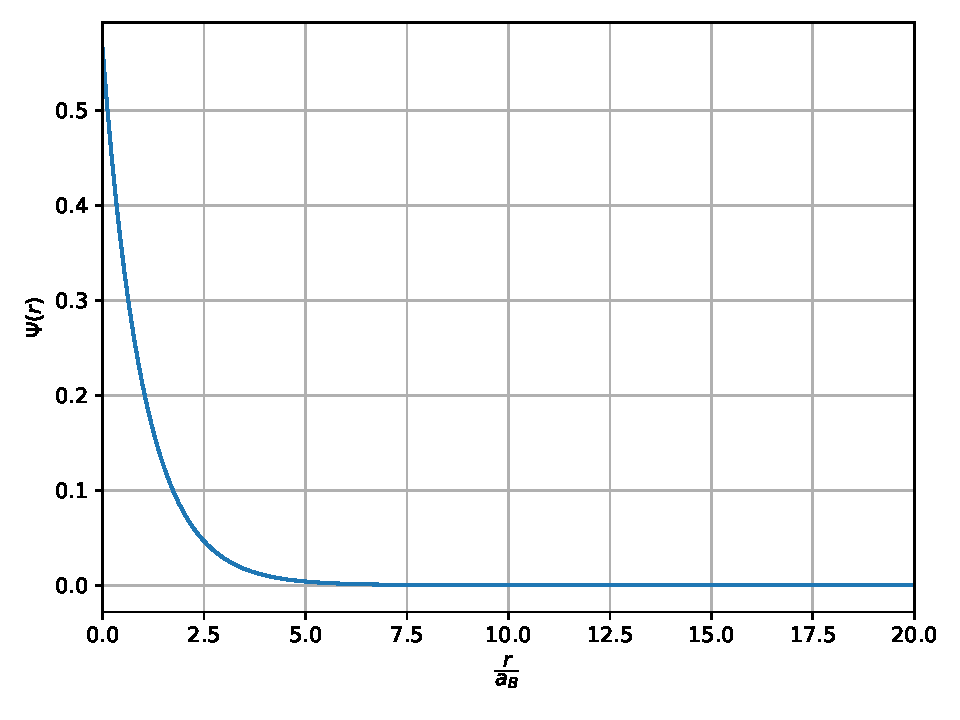
\includegraphics{build/Graph_a.pdf}
    \caption{Filterkurve der Brückenschaltung}
    \label{fig:Graph_a}
\end{figure} 

Es wurde versucht mit $ scipy$ eine Lorentzkurve der Form \eqref{eq:Lorentzkurve}, sowie eine Gaußverteilung der Form \eqref{eq:gauß} zu fitten, jedoch konnten keine Parameter, die zu den Messdaten passen gefunden werden

\begin{equation}
    f_l(v) = \frac{a}{(v^2-v_0^2)^2 + {\gamma}^2 v_0^2}
    \label{eq:Lorentzkurve}
\end{equation}

\begin{equation}
    f_g(v) = b \cdot \exp{\frac{(v-v_0)^2}{a}} \,.
    \label{eq:gauß}
\end{equation} 

Das Maximum der Spannung wird als

\begin{equation*}
    U_\text{A} = 8,1 \, \unit{\volt}
\end{equation*}

bei einer Frequenz von 
\begin{equation*}
    v_0 = 21,05 \, \unit{\kilo\hertz}
\end{equation*}
bestimmt.
Für $ v_{-} $ wir der folgende Wert ablesen
\begin{equation*}
  v_{-} = \left( 20,75 \pm 0,5 \right)\, \unit{\kilo\hertz} \text{und}
  v_{+} = \left( 23,00 \pm 0,5 \right)\, \unit{\kilo\hertz}
\end{equation*}
für $v_{+}$.
Die Güte des Selektivverstärkers wird über
\begin{equation}
  Q = \frac{v_0}{v_{+}-v_{-}}
  \label{eq:guete}
\end{equation}
berechnet, was einen Wert von $ 9,4 \pm 2.9 $ ergibt.





\subsection{Experiementelle Bestimmung der Suszeptibilität}

Es wird eine Sinusspannung mit einer Frequenz von $ 21,920 \, \unit{\kilo\hertz}$ als Speisespannung verwendet.
Die Probe liegt als Pulver vor, die Dichte $ \rho_p$ ist also geringer als es bei einem einzelnen Kristall der Fall wäre.
Deswegen wird aus dem eigentlichen Querschnitt ein realer Querschnitt $Q_{real} $ berechnet, welchen die Probe hätte, wenn sie aus einem Kristall bestehen würde.
Dazu wird die Formel \eqref{eq:Qreal} verwendet
\begin{equation}
    Q_{real} = \frac{M_p}{l \, \rho_w} .
    \label{eq:Qreal}
\end{equation}
$M_p$ ist die Masse der Probe, $\rho_w$ ist die Dichte eines Einkristalls und $l$ die Länge der Probe. \\

Die Werte für die Proben sind der der folgenden \autoref{tab:tab2} angegeben.


\begin{table}[H]
    \centering
    \caption{Stoff, Länge der Probe, Masse, Dichte und realer Querschnitt der Probe.}
    \label{tab:tab2}
    \begin{tabular}{S S S S S}
      \toprule
        {$\text{Stoff}$}&{$l \mathbin{/} \unit{\centi\meter} $}&{$\text{M}_p \mathbin{/} \unit{\gram} $}&{$ \rho_w \mathbin{/} \unit{\gram} \cdot \unit{\centi\meter}^{-3}$}&{$Q_{real} \mathbin{/} \unit{\centi\meter}^{2}$}\\
        \midrule
        {$\text{Dy}_2 \text{O}_3$} & {15,5}& {14,34}&{7,81\cite{ap07}}&{0,1189}\\
        {$\text{Gd}_2 \text{O}_3$} & {15,9}& {10,20}&{7,07\cite{ap07}}&{0,8669}\\
        {$\text{Nd}_2 \text{O}_3$} & {16,0}& {7,66 }&{7,24\cite{ap07}}&{0,6613}\\
      \bottomrule
    \end{tabular}
\end{table}


\begin{table}[H]
    \centering
    \caption{Messdaten für $\text{Dy}_2 \text{O}_3$.}
    \label{tab:tab3}
    \begin{tabular}{S S S S S S}
      \toprule
        {$ R_0 \mathbin{/} \unit{\ohm} $}&{$R_m \mathbin{/} \unit{\ohm} $}&{$ \Delta R \mathbin{/} \unit{\ohm}$}&{$ U_0 \mathbin{/} \unit{\volt}$}&{$U_m \mathbin{/} \unit{\volt}$}&{$\Delta U \mathbin{/} \unit{\volt}$}\\
        \midrule
        {2,67} & {1,145}&  {1,525}&{0,0615}&{0,0895}&{0,0280}\\
        {2,65} & {1,15} &  {1,5}  &{0,062} &{0,057} &{0,0050}\\
        {2,61} & {0,965}&  {1,645}&{0,0605}&{0,054} &{0,0065}\\
      \bottomrule
    \end{tabular}
\end{table}

\begin{table}[H]
    \centering
    \caption{Messadaten für $\text{Gd}_2 \text{O}_3$.}
    \label{tab:tab4}
    \begin{tabular}{S S S S S S}
      \toprule
        {$ R_0 \mathbin{/} \unit{\ohm} $}&{$R_m \mathbin{/} \unit{\ohm} $}&{$ \Delta R \mathbin{/} \unit{\ohm}$}&{$ U_0 \mathbin{/} \unit{\volt}$}&{$U_m \mathbin{/} \unit{\volt}$}&{$\Delta U \mathbin{/} \unit{\volt}$}\\
        \midrule
        {2,56} & {1,785}&  {0,775}&{0,058}&{0,0595}&{0,0015}\\
        {2,50} & {1,810}&  {0,690}&{0,061}&{0,0585}&{0,0025}\\
        {2,55} & {1,805}&  {0,745}&{0,062}&{0,0590}&{0,0030}\\
      \bottomrule
    \end{tabular}
\end{table}

\begin{table}[H]
    \centering
    \caption{Messadaten für $\text{Nd}_2 \text{O}_3$.}
    \label{tab:tab5}
    \begin{tabular}{S S S S S S}
      \toprule
        {$ R_0 \mathbin{/} \unit{\ohm} $}&{$R_m \mathbin{/} \unit{\ohm} $}&{$ \Delta R \mathbin{/} \unit{\ohm}$}&{$ U_0 \mathbin{/} \unit{\volt}$}&{$U_m \mathbin{/} \unit{\volt}$}&{$\Delta U \mathbin{/} \unit{\volt}$}\\
        \midrule
        {2,68} & {2,30} &  {0,38}&{0,0610}&{0,0655}&{0,0045}\\
        {2,51} & {2,38} &  {0,13}&{0,0615}&{0,0615}&{0,0000}\\
        {2,60} & {2,30} &  {0,30}&{0,0645}&{0,0630}&{0,0015}\\
        \bottomrule
    \end{tabular}
\end{table}

Die Tabellen \autoref{tab:tab3}, \autoref{tab:tab4} und \autoref{tab:tab5} zeigen die aufgenommenen Widerstände und Spannungen vor und nach dem
Einlegen der Proben sowie ihre Änderungen für die drei verschiedenen Proben.\\
Nach \eqref{eq:widsus} kann die Suszeptibilität durch $ \Delta R $ ausgrechnet werden und nach \eqref{eq:spannsussimp} über $\Delta U$.
Die Mittelwerte der Ergebnisse sind in \autoref{tab:tab6} eingetragen.


\begin{table}[H]
    \centering
    \caption{Suszeptibilitäten $\chi$ der unterschiedlichen Proben.}
    \label{tab:tab6}
    \begin{tabular}{S S S S}
      \toprule
       {Stoff} & {$\chi_{\text{R}}$} & {$\chi_{\text{U}}$} &{$\chi_{\text{theo}}$}  \\
      \midrule
      {$\text{Dy}_2\text{O}_3$}  &{$0,02271 \pm 9,2 \cdot 10^{-4}$}    &{$ 0,38346 \pm 0,30599$} &{0,02525}         \\
      {$\text{Gd}_2\text{O}_3$}  &{$0,00147 \pm 7,0 \cdot 10^{-5}$}    &{$ 0,00932 \pm 0,00249$} &{0,01370}         \\
      {$\text{Nd}_2\text{O}_3$}  &{$0,00071 \pm 2,7 \cdot 10^{-4}$}    &{$ 0,01048 \pm 0,00980$} &{0,00299}         \\
      \bottomrule
    \end{tabular}
\end{table}
